\documentclass[a4paper, 12pt, twoside]{extbook}
\usepackage[T1]{fontenc}
\usepackage[utf8x]{inputenc} %[utf8x]
\usepackage{geometry}
\usepackage{courier}
\usepackage[hidelinks]{hyperref}
\usepackage{tocbibind} %[nottoc]
\newgeometry{
left=   1.25 in,
bottom= 1.5 in,
right=  1.25 in,
top=    1 in
}
\usepackage{fancyhdr}

% Astronomycal Symbols
%\usepackage{mathabx}
\usepackage[
    starfontserif % comment for sans glyphs
    ]{starfont}

% Package for Greek alphabet
\usepackage{textalpha}

% Graphics
\usepackage{graphicx,pstricks}
\usepackage{graphics}
\graphicspath{img/}

% \usepackage{tikz}
% \usepackage{tikz-cd}
% \usepackage{pgf}
% \usepackage{pgfmath}
% \usepackage{pgfplots}
% \pgfplotsset{compat=1.14}
% \usepackage{lmodern}
% \usepackage{import}

% Package usati per il frontespizio
\usepackage{tikz}
\usepackage{pgf-pie}
\usepackage{pgfplots}
\pgfplotsset{width=7cm,compat=1.8}
\usetikzlibrary{patterns}

% Packages for lists
\usepackage{enumitem}
\setlist[itemize]{noitemsep}

% Algorithm
\usepackage{algorithm}
\usepackage{algpseudocode}  % \usepackage[noend]{algpseudocode}
\makeatletter   % to remove algorithm numbering
\renewcommand{\fnum@algorithm}{\fname@algorithm}
\makeatother
%\usepackage{algorithmic}
\usepackage{listings}

\setlength\headheight{44.2pt}
%P age Style
\usepackage{setspace}
%\setstretch{2.5} 
\doublespace

%\cfoot{\thepage}
\lhead[]{}
\rhead[]{\leftmark}

\pagestyle{fancy}{
\lhead{
\includegraphics[scale=0.3]{img/logo/hlogo.png}}
\rhead{\footnotesize{Titolo abbreviato come intestazione}}
}

% Bibliography
\usepackage{notoccite}  


% Other
\usepackage{comment}
\usepackage{amsmath}

\DeclareSymbolFont{starfontsym}{OT1}{sts}{m}{n}
\DeclareMathSymbol{\mathTerra}{\mathord}{starfontsym}{76}
\DeclareMathSymbol{\mathSun}{\mathord}{starfontsym}{115}
\DeclareMathSymbol{\mathMoon}{\mathord}{starfontsym}{100}

% Testo riempitivo
\usepackage{lipsum}


\begin{document}

    %\maketitle
    %\thispagestyle{empty}
    \frontmatter

    \cleardoublepage
\thispagestyle{empty}
\vspace*{\stretch{1}}
\begin{flushright}
\itshape <<'A forz 'e l'ambizione è chell c'avvicin 'e stell a terr>> 

        (The power of ambition is what brings the stars closer to the ground)

         Co'Sang

         %% The power of ambition is what brings the stars closer to the ground
\end{flushright}
\vspace{\stretch{2}}
\cleardoublepage
    \thispagestyle{empty}
    \chapter{Abstract} 

perché


    \chapter{Acknowledgments} 

\lipsum[1-3]

% Esempio di citazione bibliografica - vedi file "bibliography.bib"
\cite{lamport1994latex}


    {\setstretch{1}
\tableofcontents
}
    {\setstretch{1}
\listoffigures
}
    \chapter{List of Tables} 
    \chapter{List of Abbreviations and Acronyms}

 
\begin{description}[leftmargin=*, widest=DCCHTM]

    \item[AFSPC]
    Air Force Space Command
    
    \item[API]
    Application Programming interface

    \item[ARES]
    Assessment of Risk Event Statistics 

    \item[BC]
    Ballistic Coefficient

    \item[COESA]
    Committee On Extension to the Standard Atmosphere

    \item[CROC]
    Cross-section of Complex bodies

    \item[DMU]
    Drag Make Up

    \item[DOPRI]
    Dormand-Prince

    \item[DRAMA]
    Debris Risk Assessment and Mitigation Analysis

    \item[ECEF]
    Earth-Centered Earth-Fixed

    \item[ECI]
    Earth-Centered Inertia

    \item[EOL]
    End-Of-Life

    \item[ESA]
    European Space Agency

    \item[GEO]
    Geostationary Orbit

    \item[GMAT]
    General Mission Analysis Tool

    \item[HF2]
    Hyperfield 2

    \item[IAM]
    Inclination Adjust Maneuvers

    \item[JB2008]
    Jacchia-Bowman 2008

    \item[JIT]
    Just-In-Time

    \item[LEO]
    Low Earth Orbit

    \item[MASTER]
    Meteoroid and Space Debris Terrestrial Environment Reference

    \item[MIDAS]
    MASTER-based Impact flux and Damage Assessment Software

    \item[MIT]
    Massachusetts Institute of Technology 

    \item[MLTAN]
    Mean Local Time of the Ascending Node

    \item[NASA]
    National Aeronautics and Space Administration

    \item[OSCAR]
    Orbital SpaceCraft Active Removal

    \item[PSW]
    Potential Swath Width

    \item[RAAN]
    Right Ascension of the Ascending Node

    \item[RTC]
    Revisit Time Collector

    \item[SARA]
    re-entry Survival And Risk Analysis

    \item[SRP]
    Solar-Radiation Pressure

    \item[SSO]
    Sun-Synchronous Orbit

    \item[TLE]
    Two-Line Element

    \item[UTC]
    Coordinate Universal Time

    \item[VIS-NIR]
    Visible-to-Near-Infrared
    
    \item[VIS-SWIR]
    Visible-to-Short-Wave-Infrared
        
\end{description}


    \mainmatter


    \chapter{Introduction}


\section{Earth Observation and Remote Sensing}

\subsection{Hyperspectral imaging}

\section{Kuva Space}

\subsection{Company Mission}
%% subsubsection does not work
\subsection{Infrastructure}
\subsection{Distribution}
\subsection{Application}

\section{Thesis Purpose}

\section{Organization}

    \chapter{Background} \label{background_chapter}

This chapter aims to provide an overview on the fundamentals of Space Flight Dynamics that constitute the theoretical basis of this thesis, with a specific focus on Earth Observation applications in Low Earth Orbit (LEO), as well as a literature review on orbit management methods addressed by this work.



\section{Space Flight Dynamics Introduction}

Orbital Mechanics, Astrodynamics, Astronautics and Space Flight Dynamics are all titles of university courses whose principal topic is two-body orbital motion, that involves orbit determination, orbital flight time, and orbital maneuvers \cite{kluever2018space}.
In this context, a proper definition of the subject can be the following: the study of the motion of man-made objects in space, subject to both natural and artificially induced forces \cite{griffin2004space}.


\subsection{Satellite State Representations} \label{sat_state_rep_paragraph}

% There are a number of independent parameters describing the size, shape, and spatial position of an orbit.
% Six of these have become the parameters of choice to define and describe an orbit.
To define the \textit{state} of a satellite in space six quantities are required, and they may take on many equivalent forms.
Whatever the form, the collection is called either a \textit{state vector}, usually associated with position and velocity vectors, or an \textit{element set}, typically used with scalar magnitude and angular representations of the orbit called \textit{orbital elements}.
Either set of quantities completely specify the two-body orbit and provide a complete set of initial conditions for solving an initial value problem class of differential equations.
Time is always associated with a state vector and is often considered a seventh component.
State vectors and element sets are referenced to a particular coordinate frame \cite{vallado2013fundamentals}.

This thesis will use both state vectors and a specific element set.
The latter, which is also the most common one in this field, is represented by the \textit{\textbf{classical orbital elements}} \cite{brown1998spacecraft}:
\begin{itemize}
    \item Semimajor axis, \textit{a}: the orbit size is defined by one half of the major axis dimension
    \item Eccentricity, \textit{e}: the ratio of minor to major dimensions of an orbit defines the shape
    \item Inclination, \textit{i}: the angle between the orbit plane and the reference plane or the angle between the normals to the two planes
    \item Longitude of the ascending node or Right Ascension of the Ascending Node (RAAN), $\Omega$: the angle between the vernal equinox vector and the ascending node measured in the reference plane in a couterclockwise direction as viewed from the northern hemisphere
    \item Argument of periapsis, $\omega$: the angle from the ascending node to the periapsis, measured in the orbital plane in the direction of spacecraft motion. The ascending node is the point where the spacecraft crosses the reference plane headed from south to north. the line of nodes is the line formed by the intersection of the orbit plane and the reference plane
    \item True anomaly, $\nu$: the sixth element locates the spacecraft position on the orbit
\end{itemize}

%---------IMMAGINI---------

This thesis work makes also use of the \textit{argument of latitude, u}, which is the angle measured between the ascending node and the satellite's position vector in the direction of satellite motion.
A relation that is always valid exists between classical orbital elements and the argument of latitude \cite{vallado2013fundamentals}:
\begin{equation} \label{eq:argl}
    u = \omega + \nu
\end{equation}
One more element that is often used is the \textit{mean anomaly, M}, which is the angle between the periapsis of an orbit and the position of an imaginary body that orbits in the same period as the real one but at a constant angular speed (circular orbit).
The angular speed assigned to the imaginary body is the satellite's average angular velocity over one orbit, and is called \textit{mean motion, n} \cite{ridpath2012dictionary}.

This research utilizes also another element set which results necessary to address case studies of past missions: the \textit{Two-line element set} (TLE).
A two-line element consists of a satellite identifier, an epoch, six orbital elements and a \textit{B*} term related to the ballistic coefficient \cite{riesing2015orbit}.
These elsets are available to the general public through Air Force Space Command (AFSPC) \cite{vallado2013fundamentals}.

The elements of a TLE are shown in equation \ref{eq:tle} \cite{vallado2013fundamentals}, where:
\begin{itemize}
    \item[-] the bars on  the mean motion and semimajor axis denote \textit{Kozai mean values} 
    \item[-] the numerators of the first two elements of the second line represent mean motion rate and acceleration
    \item[-] $\frac{c_D A}{m}$ corresponds to the inverse of the \textit{ballistic coefficient, BC}
    \item[-] $\rho_0$ is the atmospheric density at perigee of the orbit
    \item[-] $R_\mathTerra$ defines an Earth Radius of 6378.135 km
    \item[-] the epoch is expressed in Coordinate Universal Time (UTC)
\end{itemize}

\begin{equation} \label{eq:tle}
    \begin{split}
        \bar{n}=\sqrt{\frac{\mu}{\bar{a}^{3}}} \;\;\;\;\;\;\;\;\;\; e \;\;\;\;\;\;\;\;\;\; i \;\;\;\;\;\;\;\;\;\; \Omega \;\;\;\;\;\;\;\;\;\; \omega \;\;\;\;\;\;\;\;\;\; M \\
        \frac{\dot{n}}{2} \;\;\;\;\;\;\;\;\;\;\;\; \frac{\ddot{n}}{6} \;\;\;\;\;\;\;\;\;\;\;\; B^* = \frac{1}{2} \frac{c_D A}{m} \rho_0 R_\mathTerra \;\;\;\;\;\;\;\;\;\;\;\; UTC
    \end{split}
\end{equation}


\subsection{Reference Frames}
Two types of reference frames are adopted by this research: the geocentric-inertial coordinate system and the geographic-body-fixed system.
The origin of both systems is the center of mass of the central body, which in all case studies of this work is the Earth.
They will therefore be labeled Earth-centered inertial (ECI) and Eart-centered Earth-fixed (ECEF) coordinate frames, respectively.


\subsubsection{Earth-centered inertial}
The ECI system is shown in FIGURE???.
The equatorial plane is the reference plane.
The X axis is the vernal equinox vector, and the Z axis is the spin axis of the Earth; north is positive.
The axes are fixed in inertial space or fixed with respect to the stars \cite{brown1998spacecraft}.


\subsubsection{Earth-centered Earth-fixed}
FIGURE shows a representation of the ECEF reference frame.
The system is Earth-centered and fixed to the rotating Earth \cite{vallado2013fundamentals}.
Considering the ECI, the Z axis is the same, while the X axis always points towards the Greenwich meridian.
Satellite ground track is commonly plotted in this coordinate system \cite{brown1998spacecraft}.


\subsection{Two-Body Problem} \label{twobody_par}
The two-body problem is an indispensable theory to soak up the concepts of astrodynamics \cite{vallado2013fundamentals}.
The Newton's law of universal gravitation (equation \ref{newton_law_eq}) states that all celestial bodies are attracted to each other by a force proportional to the product of their masses and inversely proportional to the square of the distance between their centers of mass.
\begin{equation} \label{newton_law_eq}
    F_g = \frac{M m G}{r^2}
\end{equation}
$G$ is the \textit{universal gravitational constant}, while the other parameters clearly represents the masses and the distance.
The motion of every particle in the universe is therefore determined by an infinite network attractive forces to all celestial bodies.

A real study of this scenario would be unfeasible, but since the motion of a spacecraft is dominated by one central body at time, is possible to define some plausible assumptions which lead to a simplification of the problem \cite{brown1998spacecraft}.
\begin{enumerate}
    \item The motion of the satellite is governed by attraction to only one central body.
    \item The mass of the spacecraft can be neglected with respect to the central body one.
    \item The two bodies are spherically symmetrical with uniform density.
    \item Only gravitational and centrifugal forces act on the bodies, along the line of their centers. 
\end{enumerate}
Under these assumptions, it is possible to develop a second-order, nonlinear, vector, differential equation called the \textit{two-body equation} \cite{vallado2013fundamentals}:
\begin{equation} \label{kepler_eq}
    \ddot{\vec{r}} + \frac{\mu}{r^3}\vec{r} = 0
\end{equation}
where $\mu$ is equal to the product between the central body and the universal gravitational constant $G$.


\subsection{Orbital Perturbations} \label{perturbations}
Orbital perturbations are deviations from a normal, idealized, or undisturbed motion.
Introducing an alteration from two-body problem assumptions, the actual motion will vary due to perturbations caused by other bodies, and additional forces not considered in Keplerian motion \cite{vallado2013fundamentals}.
This subsection provides an overview of the main perturbations for an Earth orbiting spacecraft.


\subsubsection{Earth's Gravity Field}
Spinning celestial bodies are nor perfect spheres, but they are much more similar to oblate spheroids.
For such a planet, the spin axis can be considered as the axis of rotational symmetry and the gravitational field will vary with the latitude as well as radius.
The planet's oblateness provides a rotationally symmetric perturbation $\Phi$, which does not depend on the longitude \cite{curtis2020orbital}.

In particular, $\Phi$ is given by an infinite series characterized by the so-called \textit{zonal harmonics} $J_k$ of the planet of reference.
Considering a spherical coordinate system for convenience, with origin at the planet's center of mass and third axis as the axis of rotational symmetry,
in this series, shown in equation \ref{eq:harmonics_series}, $r$ and $\phi$ are the distance from the origin and the polar angle respectively, $\mu$ is the Earth's standard gravitational parameter, $R$ the equatorial radius and $P_k$ represent the Legendre polynomials \cite{curtis2020orbital}.
\begin{equation} \label{eq:harmonics_series}
    \Phi (r,\phi) = \frac{\mu}{r} \sum_{k=2}^{\infty} J_k \left(\frac{R}{r} \right)^k P_k (\cos{\phi})
\end{equation}
The zonal harmonics are non-dimensional quantities which are evaluated from satellite observation mission around the planet.
The summation starts from $k = 2$, and the Earth's set of zonal harmonics is highly dominated by $J_2$.
Taking into account only $J_2$ and starting from equation \ref{eq:harmonics_series}, it is possible to derivate the perturbing gravitational acceleration due to the respective zonal harmonic \cite{curtis2020orbital}:
\begin{equation} \label{eq:j2_acc}
    \vec{a}_{J_2} = \frac{3}{2} \frac{J_2 \mu R^2}{r^4} \left[\frac{x}{r}\left(5 \frac{z^2}{r^2} - 1 \right)\hat{\textbf{i}} + \frac{y}{r}\left(5 \frac{z^2}{r^2} - 1\right)\hat{\textbf{j}} + \frac{z}{r}\left(5 \frac{z^2}{r^2} - 3\right)\hat{\textbf{k}} \right]
\end{equation}

The right ascension $\Omega$ and the argument of perigee $\omega$ are significantly affected by oblateness \cite{curtis2020orbital}.
% Their variation in time is described by equations \ref{eq:5} and \ref{eq:6} respectively \cite{curtis2020orbital}:
% \begin{equation} \label{eq:5}
%     \dot{\Omega} = - \left[\frac{3}{2} \frac{\sqrt{\mu} J_2 R^2}{(1-e^2)^2 a^{7/2}}\right]\cos{i}
% \end{equation}
% \begin{equation} \label{eq:6}
%     \dot{\omega} = - \left[\frac{3}{2} \frac{\sqrt{\mu} J_2 R^2}{(1-e^2)^2 a^{7/2}}\right] \left(\frac{5}{2} \sin^2{i} - 2\right)
% \end{equation}

It is necessary to underline that the Earth's gravitational field vary not only with latitude but also with longitude due to irregularities in geometry and mass distribution \cite{curtis2020orbital}.
However, with negligible approximation, it is definitely reasonable to consider only oblateness with $J_2$ effects in LEO missions, which is the major force for this range of altitudes, second only to Earth's gravity \cite{brown1998spacecraft}.
In light of the above, this thesis will take into account only $J_2$ forces with respect to the Earth's gravity field perturbations.


\subsubsection{Atmospheric Drag}
The residual atmosphere present at a few hundred kilometers of altitude strongly influences the motion of satellites in LEO.
The basic equation of the perturbing specific force (force per unit mass) due to drag is the following \cite{vallado2013fundamentals}:
\begin{equation} \label{eq:drag_acc}
    \vec{a}_{drag} = - \frac{1}{2} \frac{C_D A}{m} \rho V_{rel}^{2} \frac{\vec{V_{rel}}}{|\vec{V_{rel}}|}
\end{equation}
In equation \ref{eq:drag_acc}, $\frac{m}{C_D A}$ is again the ballistic coefficient, that already appeared in the TLE representation (equation \ref{eq:tle}):
$m$ is the mass of the spacecraft, $A$ represents the cross-sectional area of the satellite with respect to the atmosphere and $C_D$ is the drag coefficient, a dimensionless parameter which takes into account every aerodynamic configuration aspect of the body with respect to the drag forces \cite{sadraey2009drag}.
The value of the drag coefficient for satellites in the upper atmosphere is generally around 2.2 \cite{vallado2013fundamentals};
this number has been considered for all the case studies of the thesis.
Finally, the velocity vector $\vec{V_{rel}}$ is relative to the atmosphere, as well as the cross section.

The main effects provided by aerodynamic drag are changes in the semimajor axis and eccentricity of the orbit and an accurate description of the atmospheric properties is crucial for the evaluation of drag on satellites \cite{vallado2013fundamentals}.
However, uncertainties in the time variance of upper atmosphere make perfect prediction of spacecraft drag impossible \cite{brown1998spacecraft}.
More in depth, the density changes because of a complex interaction between three factors: the nature of the atmosphere's molecular structure, the incident solar flux, and geomagnetic interactions.
Several atmospheric models can be found in literature, either static or time-varying.
The static ones are less accurate, but definitely simpler than the time-varying models, thanks to the assumption of all constant parameters \cite{vallado2013fundamentals}.
This thesis exploits three different models, depending on the applications addressed in the case studies.

The first model considered by this research is static: the exponential model, valid in the range of altitudes between 0 and 1000 km.
It assumes a spherically symmetrical distribution of particles of the atmosphere, in which the density decreases exponentially with increasing the altitude according to equation \ref{eq:exp_model} \cite{vallado2013fundamentals}
\begin{equation} \label{eq:exp_model}
    \rho = \rho_0 \exp{\left[- \frac{h - h_0}{H}\right]}
\end{equation}
where $\rho_0$ and $h_0$ represent a reference density and altitude respectively and $H$ is the scale height.

The second atmospheric model, still static, is the Standard Atmosphere published in 1976 by the U.S. Committee on Extension to the Standard Atmosphere (COESA), valid drom 0 to 1000 km of altitude.
It is an ideal, steady-state model of the Earth's atmosphere at a latitude of $45^{\circ}$N in moderate solar activity conditions \cite{vallado2013fundamentals}.

Finally, Jacchia-Bowman 2008 (JB2008) is an empirical time-varying atmospheric density model. It revises and improves the earlier Jacchia-Bowman 2006 which is based on the diffusion equations of the Jacchia 71 model.
JB2008 takes into account factors like solar irradiances, computed from driving solar indices based on orbit-based sensor data.
Density variations are described by semiannual density equations based on 81-day average solar indices, as well as from temperature equations that include corrections for diurnal and latitudinal effects.
Geomagnetic effects are modeled too.
The model is validated in the altitude range of 175 to 1000 km through comparisons with accurate daily density drag data previously collected for numerous satellites, existing atmospheric models and other measurements from several Earth orbiting satellite missions \cite{bowman2008jb2006,bowman2008new}.


\subsubsection{Third-Body Perturbations}
All the orbital elements are periodically affected by the gravitational forces of the Sun and the Moon.
Similarly to what is triggered by the Earth's equatorial bulge, they apply an external torque to the orbits and cause the angular momentum to rotate.
This perturbation is highly negligible in LEO, where the main effects are provided by $J_2$ and aerodynamic drag \cite{wertz2009orbit}.
However, low Earth orbits characterized by a constant geometry with respect to the perturbing body can be affected by emphasized long-period effects.
This is the case of Sun-synchronous orbits (SSO), for which the constant pattern with the Sun causes a long-term phenomenon of variation of the inclination (around 0.05 degrees per year) \cite{giacaglia1994long}.
Although this number might appear meaningless, inclination is critical to SSO, as will be explained in paragraph \ref{sso_paragraph}.


\subsubsection{Solar-Radiation Pressure}
The last perturbation treated by this thesis is the solar-radiation pressure (SRP), which induces periodic variations in all the orbital elements.
SRP generally becomes significant above 800 km of altitude, as drag becomes less important. Below this threshold, it might be neglected \cite{wertz2009orbit}.
The perturbing acceleration can be approximated by the following equation \cite{vallado2013fundamentals}
\begin{equation} \label{eq:srp_acc}
    \vec{a}_{SRP} = - \frac{p_{SRP} c_{R} A_{\mathSun}}{m_{sat}} \frac{\vec{r}_{\mathTerra \mathSun}}{|\vec{r}_{\mathTerra \mathSun}|}
\end{equation}
$p_{SRP}$ is the solar pressure, which is a quantity representing the change in momentum per unit area, derived by the ratio between the solar flux and the speed of light.
The reflectivity, $c_R$, a value between 0.0 and 2.0, models the type of interaction between radiation and surface exposed to the Sun, $A_{\mathSun}$ \cite{vallado2013fundamentals}.
$m_{sat}$ is trivially the mass of the satellite.


\subsection{Mean Orbital Elements}
The previous subsection has described how orbital perturbations generate continuous variations and oscillations in the orbit elements.
The values of the elements at a single point in time, which are periodically and secularly affected by the perturbing forces, are called \textit{osculating elements}.
On the other side, it is possible to define the \textit{mean orbit elements}, which represent the average motion over a span of time \cite{wertz2009orbit}.
In this way it is possible to obtain a representation of the orbital motion removing short and long-periodic effects induced by perturbations.
And for most operational purposes, conversion from osculating to mean elements is indispensable \cite{walter1967conversion}.
Indeed, applications addressed by this work, like station-keeping and differential drag, require the secular behavior of the satellite to be implemented.

The oblateness of the Earth is the main guilty of periodic effects, provoking variations in all osculating elements, as well as all the other zonal harmonics.
On the other hand, only even zonal gravitational harmonics and atmospheric drag give raise to secular effects in osculating elements, which are constant or non-periodic.
Aerodynamic drag secular perturbation plays a crucial role in LEO \cite{der1996conversion}.

Figure \ref{osc_vs_mean_sma} shows the comparison between osculating and mean semi-major axis of a LEO satellite motion over the course of four months.
The orbital decay induced by the atmospheric drag secular effect is evident, as well as the periodic consequences of $J_2$ perturbation.
\begin{figure}[h]
    \centering
    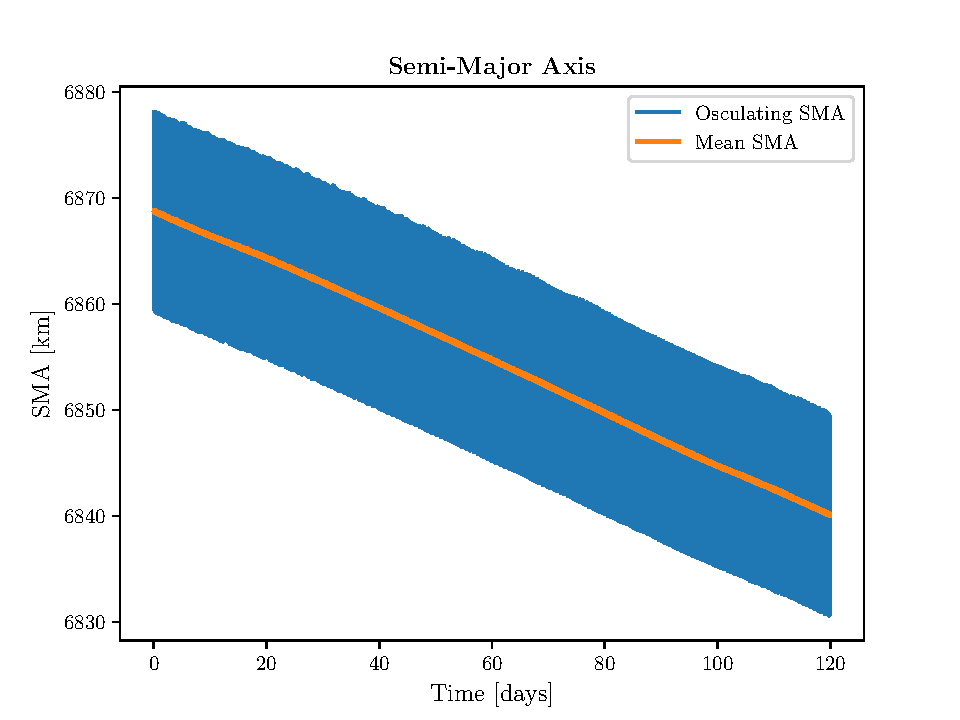
\includegraphics[scale=0.9]{img/osc_vs_mean.pdf}
        \caption{Osculating vs. mean semi-major axis for a LEO satellite under atmospheric drag and $J_2$ perturbations.}
    \label{osc_vs_mean_sma}
\end{figure}

Several perturbation techniques have been proposed to perform the conversion between osculating and mean elements. 
Brouwer and Kozai works were ones of the first methods appeared in literature, both consisting of first order solutions which take into account the Earth's asphericity but neglect drag effects \cite{arnas2022analytic}.
This thesis uses a refinement of Brouwer's approach, suggested by Lyddane, which solves zero eccentricity and inclination singularities that are involved in the original theory.
Moreover, the algorithm will account only first order $J_2$ terms \cite{schaub2002analytical}.


\subsection{Orbit Propagation} \label{orbit_prop_paragraph}
Orbit propagation is the principal problem in perturbation analysis.
There are numerous methods to analyse the perturbing force models, and they can be classified in three categories  \cite{vallado2013fundamentals}:
\begin{itemize}
    \item \textit{Special perturbation techniques}: they are numerical solutions, and they represent the most accurate way.
    \item \textit{General perturbation techniques}: they are analytical methods based on approximations, which means the accuracy is lower, but the computation is speeded up.
    \item \textit{Semianalytical techniques}: these techniques combine the best features of the previous categories, which means both good accuracy and computational efficiency.
\end{itemize}
The technique selected to design the tools shown in chapter \ref{chapter_tools} falls into the first category.
Actually, the purposes of the thesis would even be achieved by a general perturbation method, saving time in the calculation phase.
Indeed, there are not strict requirements of accuracy, since the research look of this work.
However, a special perturbation technique has been chosen in order to provide more valuable tools which might be useful in the advanced stages of future Kuva Space missions.
Furthermore, this is also a reasonable choice due to the long-time propagations needed by operations that will be discussed later.


\subsubsection{Cowell's Technique}
The Cowell's special perturbation technique is implemented in the algorithms produced by this thesis.
The idea of this method is to add the perturbing accelerations to the two-body equation:
\begin{equation} \label{cowell_eq}
    \ddot{\vec{r}} = - \frac{\mu}{r^3}\vec{r} + \vec{a}_p
\end{equation}
$\vec{a}_p$ represents the total acceleration given by the perturbing forces, like that ones seen in paragraph \ref{perturbations} (e.g., equation \ref{eq:drag_acc}), while $\vec{r}$ is clearly the state vector of the satellite.
Equation \ref{cowell_eq} is called \textit{Cowell's formulation}.
This second-order differential equation of motion needs a numerical integration method to be solved \cite{vallado2013fundamentals}.


\subsubsection{Dormand-Prince Method}
The topic of numerical integration would require in-depth treatment due to its complexity, but only the method used by this work is briefly described in the next lines.
The propagators developed to accomplish the purposes of the thesis take advantage of an eigth-order \textit{Dormand-Prince} (DOPRI) method to solve the Cowell's equation.
It is a single-step and variable step-size integrator.
This means that it determines the subsequent steps exclusively from the information of the latest previous step.
On the other hand, while fixed-step techniques divide the propagation into equal time steps, variable step-size algorithms dynamically adjust the step size.
This is carried out including tolerance criteria to identify the accuracy at each step by considering two methods \cite{rocha2018numerical}.
For instance, the thesis uses a DOPRI$8_{(5,3)}$, which means order 8 for the integration, with a 5th order error estimator combined with a 3rd order correction.



\section{Specialized Orbits}
\textit{Specialized orbits} are the results of specific orbital features selected during the design of a mission, which can be simply related to the orbit period or, more commonly, to one of the main orbit perturbations \cite{wertz2009orbit}. 
In this section, two special Earth orbits will be analysed, both of interest for the purposes of the thesis.
In fact, in general methods, the higher the propagation times, the lower the accuracy.


\subsection{Sun-Synchronous Orbit} \label{sso_paragraph}
Sun-synchronous orbits are specialized orbits characterized by a constant geometry with the Sun over time \cite{vallado2013fundamentals}. 
They are used for several reasons, from technical needs like that ones deriving from thermal and electric power subsystems of the spacecraft to application requirements such as remote sensing.
Indeed, a constant Sun angle is very precious for missions working with electro-optical sensors \cite{brown1998spacecraft}.
This is the case, for instance, of hyperspectral technology. 

An SSO can be obtained by matching the Westward motion of the line of nodes (\textit{regression of the nodes}) to the solar motion projected on the equator, like shown in equation \ref{sso_raan} \cite{brown1998spacecraft}.
\begin{equation} \label{sso_raan}
    \dot{\Omega} = 360^{\circ} / 365.242\;days = 0.9856\;^{\circ}/day 
\end{equation}
This will allow the satellite's line of nodes to keep a constant angular separation with respect to the Sun.
This separation can be achieved with very good approximation only considering the dominant cause of the secular motion of RAAN: $J_2$ perturbation.  
The secular behavior of $\Omega$ induced by the oblateness is function of semi-major axis, eccentricity and inclination and is given by the following formula \cite{vallado2013fundamentals}:
\begin{equation} \label{raan_variation}
    \dot{\Omega}(a,e,i) = - \frac{3n R_{\mathTerra}^2 J_2}{2a^2 (1-e^2)^2} \cos{i}
\end{equation}
Equations \ref{sso_raan} and \ref{raan_variation} suggest that to achieve the proper $\dot{\Omega}$ of an SSO, the inclination has to be more than 90$^\circ$ (\textit{retrograde orbit}), so that the term $\cos{i}$ will become negative \cite{wertz2009orbit}.
As for the other two variables, eccentricity is generally supposed to be near-zero because low-Earth orbits usually imply very small values of $e$.
Hence, with the assumption of $e=0$, an SSO will be characterized by a direct relationship between $a$ and $i$.
Figure \ref{inc_h_sso} shows the range of inclinations and altitudes that would provide the proper regression of nodes.
\begin{figure}[h]
    \centering
    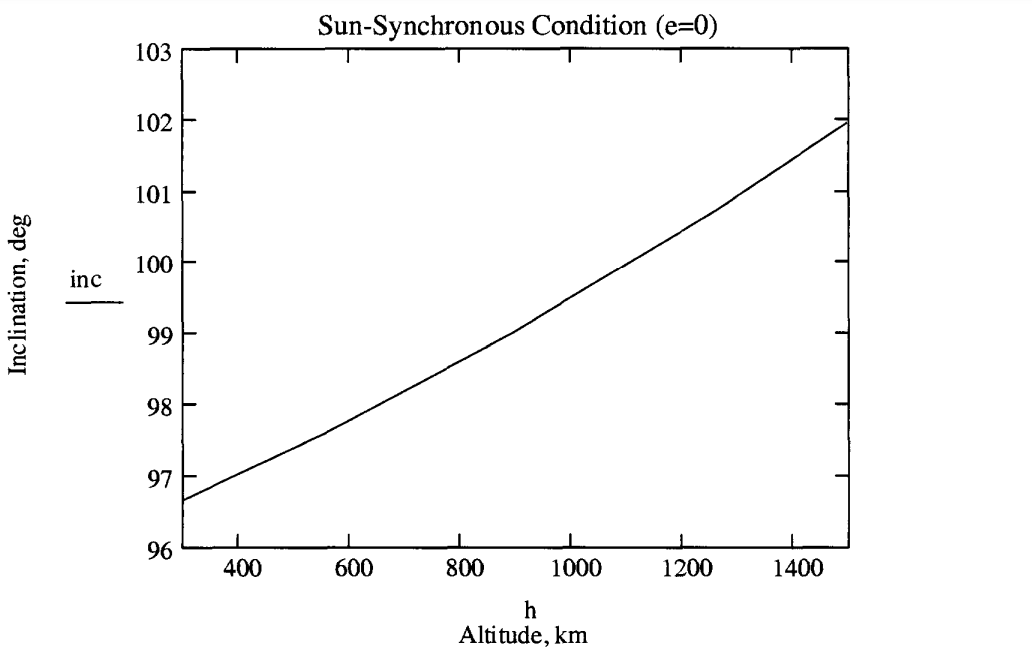
\includegraphics[scale=0.5]{img/inc_vs_h_sso.png}
    \caption{SSO condition: inclination vs. altitude ($e=0$) \cite{brown1998spacecraft}.}
    \label{inc_h_sso}
\end{figure}

In addition, it is possible to select the initial value of the RAAN between 0 and 360 degrees according to the mission requirements for example \cite{vallado2013fundamentals}.
The angle between the ascending node and the direction of the Sun is commonly labeled like \textit{Mean Local Time of the Ascending Node} (MLTAN), because of the relative time to the noon meridian.
This is a crucial design parameter because, while for an arbitrary orbit the MLTAN would continually change, for a Sun-synchronous orbit it will remain constant \cite{boain2004ab} (not only at the nodes, but at any latitude).

In order to provide a better understanding of the concepts, figure \ref{sso_curtis} shows an example of an SSO with an LTAN of 15:00.
\begin{figure}[h]
    \centering 
    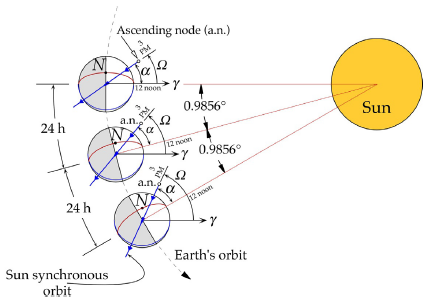
\includegraphics[scale=1]{img/sso_curtis.png}
    \caption{Sun-synchronous orbit 15:00 LTAN illustration \cite{curtis2020orbital}.}
    \label{sso_curtis}
\end{figure}


\subsection{Repeat-Groundtrack Orbit} \label{repeat_groundtrack}
The peculiarity of a \textit{repeat-groundtrak orbit} is the repetitive transit of the satellite to the same location relative to the surface of the Earth after a certain time interval \cite{wertz2009orbit}.
Hence, they are used by missions which need to periodically revisit a specific point on the Earth \cite{vallado2013fundamentals}, playing an interesting role in remote sensing applications.

Considering $j$ orbit periods and the relative $k$ days spent, an orbit is repetitive if and only if the ratio $Q$ between $j$ and $k$ is a rational number, where $Q$ represents the number of orbits per day.
This means that $j$ and $k$ are integer and prime to each other.
For instance, if a satellite performs 15.25 orbits per day, it will make a 4-day repeating ground track, because the respective rational $Q$ is given by $j=61$ orbits in $k=4$ days \cite{wertz2009orbit}.
$k$ is typically known as the \textit{revisit time} of the spacecraft, defined as the time elapsed between two successive observations of the same ground point \cite{luo2017novel}.
It is necessary to underline that the effects of perturbations should be taken into account in order to obtain accurate repetition properties, since the actual period appears more complex \cite{wertz2009orbit}. 

In light of the above, it can be easily understood that the minimum achievable revisit time for a generic orbit is 1 day.
However, mission objectives might require shorter revisit times.
The solution to this issue is the design of a constellation of satellites, as will be discussed later.



\section{Satellite Constellations}
A satellite constellation can be defined as a group of similar satellites, with comparable functions and properties, designed to operate in similar, complementary orbits to undertake common objectives, under shared control \cite{wood2003satellite}.
In the context of this thesis, Earth-orbiting constellations are of notable interest thanks to the global coverage of the world they can enhance with respect to a single satellite mission. 
In recent years, the availability of smaller, lower-cost satellites, and the easier access to space have led to a drastic evolution in the design of constellations.
Thanks to this trend, applications like observation, communication and navigation have drastically expanded their potential \cite{wertz2009orbit}. 

\subsection{Walker Delta Constellation}
\textit{Walker constellations} are the most symmetric of the satellite pattern families.
The \textit{Walker Delta} is the most popular model within the latter, which is also the one selected for the future Kuva Space constellation.
This satellite pattern can be fully determined through four parameters. 
$T$ represents the total number of satellites, uniformly distributed in each of the $P$ orbit planes.
$i$ is the inclination of the orbits, which is supposed to be the same for all.
The last term is $F$, and is defined as the relative spacing between satellites in adjacent planes.
In a constellation $\Delta \phi$ is defined like the \textit{phase difference}, which is the angle in the direction of motion from the ascending node to the nearest satellite at a time when a satellite in the next most westerly plane is at its ascending node.
$\Delta \phi$ must be an integral multiple of $360^\circ / T$, and can be any integer number from $0$ to $P-1$: this value is $F$ \cite{wertz2009orbit}.
\begin{equation} \label{walker_delta_notation}
    i : T/P/F
\end{equation}
Equation \ref{walker_delta_notation} shows the shorthand notation used to indicate a Walker Delta constellation.

An example of a Walker Delta configuration is displayed in figure \ref{walker_delta_representation}.
\begin{figure}[h]
    \centering
    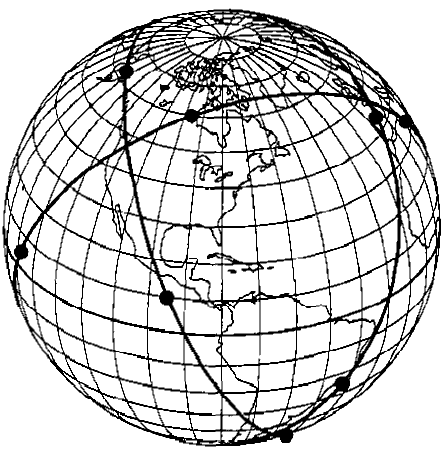
\includegraphics[scale=0.5]{img/walker_delta.png}        
    \caption{Illustration of a 65:15/3/2 Walker Delta configuration \cite{wertz2009orbit}.}
    \label{walker_delta_representation}
\end{figure}
The complete symmetry in longitude is one of its main advantages.
In addition, there is a finite number of Walker constellations, and all of them can be identified and investigated.
This allows the mission designer a full analysis of the constellation on every aspect of interest \cite{wertz2009orbit}. 

% \subsection{Constellation Design}

\section{Constellation Orbit Management}
Over the life of a space mission, the need to adjust or maintain the orbit elements might arise. In general, orbit maintenance is required because of two main reasons:
targeting to reach an end orbit or position, or to maintain absolute or relative orientations \cite{wertz2009orbit}.

This thesis focuses on two different phases of constellation orbit management, proposing a possible strategy for the main case study. 
The first maneuver addresses the \textit{initial orbit phasing} of a satellite fleet after the deployment from the launcher.
The plan is to dispose the spacecraft into the desired pattern through a \textit{differential drag} method.
The second action consists of the \textit{relative station-keeping}.
It aims to maintain the relative positions of the vehicles within the same orbit, taking advantage of low-thrust propulsion systems.

Downstream of this two-step strategy, an analysis of space debris mitigation is carried out in order to assess the importance of collision avoidance in a satellite constellation. 


\subsection{Initial Orbit Phasing (Differential Drag)}
The initial orbit phasing treated by this work consists of the achievement of the desired formation of a group of satellites deployed within the same orbit.
In particular, the final scheme considered by the thesis is composed by a nominal altitude (lower than the deployment's one) and a symmetric pattern with equal relative angular separation between the spacecraft.
A differential drag method is proposed to accomplish this purpose.

Differential drag can be defined as the difference in atmospheric drag acting on each of a couple of satellites.
Assuming that the spacecraft travel through similar atmospheric density areas, the differential drag is almost fully determined by differences in ballistic coefficient of them \cite{leonard1991formationkeeping}.
Considering identical satellites, and remembering that BC depends on the area perpendicular to the velocity vector, differential drag can be achieved controlling the attitude of the body, leading to different values of surface exposed to the aerodynamic flux. 

To clarify ideas and simplify the problem, only two configurations will be identified as shown in figure \ref{low_vs_high_dragmode_fig}: low-drag and high-drag modes.
\begin{figure}[h]
    \centering
    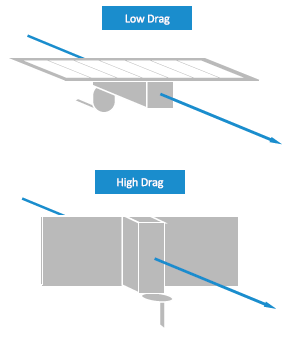
\includegraphics[scale=1]{img/low_vs_high_dragmode.png}
    \caption{Low drag vs. high drag mode of a generic satellite shape \cite{foster2018differential}.}
    \label{low_vs_high_dragmode_fig}
\end{figure}

Moreover, the satellite on the lower orbit will be indicated as the \textit{leading satellite}, whereas the other one \textit{trailing satellite}.
Supposing of using differential drag only to equalize the altitudes, with both spacecrafts travelling in low-drag profile, the trailing satellite shall be set to high-drag mode until the leader's orbit is reached.
Indeed, the acceleration of its motion is the same as if the air drag force, reversed, were pushing the satellite. 
This phenomenon is known as \textit{satellite paradox} \cite{mills1959satellite}. 

Several applications can take advantage from differential drag. 
It was first proposed for \textit{formationkeeping} to keep a satellite in a specific position with respect to another.
Even rendezvous maneuver strategies have been combined with differential drag actions.
This method has also been selected for collision avoidance scenarios \cite{foster2018differential}.

What is of huge interest for the purposes of the thesis is the experience provided by Planet company (formerly Planet Labs).
They applied differential drag control to fleets of propulsion-less satellites deployed in the same orbit with successful results for several missions.
The goal of Planet's controller was to bring all the spacecrafts at the same altitude and perform phasing with only differential drag after deployment from launcher.
Three examples of constellation phasing are shown in figure \ref{phasing_examples_figure}.
\begin{figure}[h]
    \centering
    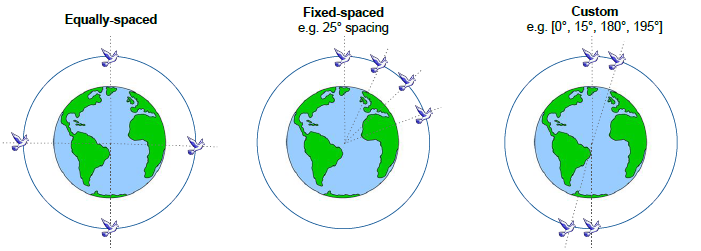
\includegraphics[scale=1]{img/phasing_examples.png}
    \caption{Generic cases of desired relative placement of four satellites \cite{foster2018differential}.}
    \label{phasing_examples_figure}
\end{figure}
The initial conditions subsequent to the deployment contain small but significant variations in SMA: achieving the same orbital altitude means zero-relative speed between them.
On the other hand, the phasing aims to symmetrically separate the vehicles in terms of angular distance, along the same orbit. 
Once the desired constellation pattern is achieved, the differential drag control continues to operate as station-keeping to maintain the formation, since the propulsion-less nature of the satellites \cite{foster2018differential}.

Based on the Planet's controller, this thesis proposes an algorithm for the phasing of a group of satellites after the initial dispersion from the launcher only using differential drag. 


\subsection{Absolute Station-Keeping} \label{station_keeping_par}
Station-keeping can be defined as the procedure of controlling a satellite in order to maintain its position within a specific imaginary box or with respect to inertial space or other spacecraft. 
In constellation maintenance, the only goal is to keep the relative placement between satellites.
Orbit perturbations and variations in initial conditions for each vehicle are the major causes which make necessary maintenance maneuvers.
A long-lived LEO constellation must principally fight the atmospheric drag in order to avoid orbit decay.

The strategy addressed by the thesis follows the approach of constantly negating the perturbing force, which requires continuous propellant usage.
More in detail, each vehicle is kept in a well-defined mathematical box under \textit{absolute station-keeping}.
The idea is to periodically put back the $\Delta V$ taken out by drag.
This is equivalent to keep the satellite in a box by letting it drift to one side of the box, hitting it with a thruster, letting it drift across the box and back, and repeat the cycle, as shown in figure \ref{sk_box_figure}
The objective is to maintain a desired pattern as illustrated by figure \ref{constellation_sk_boxes_figure}.
Station-keeping boxes must typically be 10 to 50 kilometers long, and accounting for low-thrust propulsion systems, this strategy will need a large number of small burns \cite{wertz2009orbit}.

\begin{figure}[h]
    \centering
    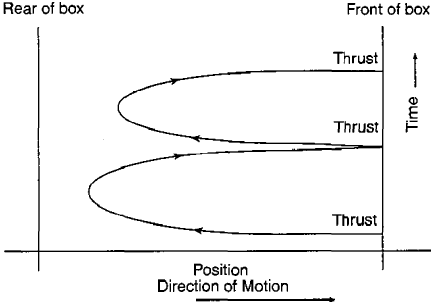
\includegraphics[scale=0.7]{img/sk_box.png}
    \caption{Satellite's drift in the station-keeping box \cite{wertz2009orbit}.}
    \label{sk_box_figure}
\end{figure}

\begin{figure}[h]
    \centering
    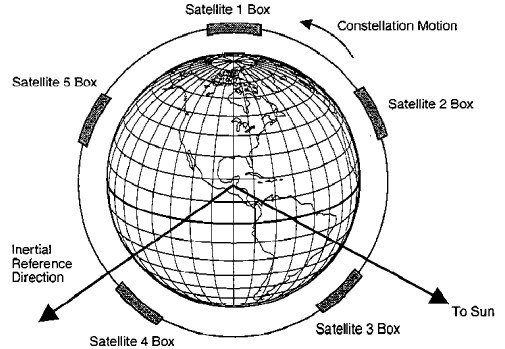
\includegraphics[scale=0.7]{img/constellation_sk_boxes.png}
    \caption{Absolute station-keeping of a group of satellites within the same orbit \cite{wertz2009orbit}.}
    \label{constellation_sk_boxes_figure}
\end{figure}

In conclusion, this thesis takes into account the regular execution of annual Inclination Adjust Maneuvers (IAM) and frequent Drag Make Up (DMU) maneuvers to counteract perturbing effects \cite{johnson2014maintaining}.
The simulations of these scenarios, which naturally involve forces generated by thrusters, rely on the \textit{Edelbaum-Kechichian} formulas.

\subsubsection{Edelbaum-Kechichian Theory}
An analytic solution for the optimum low-thrust transfer between inclined circular orbits of different radius is provided by the equations of Edelbaum reformulated by Kechichian in 1992 \cite{edelbaum1961propulsion, kechichian1992reformulation}.
This thesis takes advantage of this theory to compute $\Delta V$, burning time and related acceleration needed to satisfy the requirements of station-keeping.

The problem assumes only tangential and out-of-plane acceleration, and circular orbits during the transfer ($e = 0$).
These assumptions are widely acceptable in this context, because all the case studies of this research are characterized by near-circular orbits, and the thrust direction of the satellites is ideally intended to be parallel to the velocity vector.

The first input parameter is the thrust force acceleration $f$, deriving from the ratio between the thrust provided by the thruster and the spacecraft mass, which is broken down into three mutually orthogonal components:
the first one is tangential to the velocity vector of the satellite, the second component is normal to the orbital plane, and the last one is in the out-of-plane direction.
 
They are expressed in terms of two angles: 
$\alpha$ is the angle between the velocity vector and the component of the thrust vector in the plane of the orbit,
while $\beta$ represents the angle between the thrust vector and the plane of the orbit \cite{edelbaum1961propulsion}.
\begin{equation} \label{acceleration_thrust_components}
    f_T = f \cos{\beta} \cos{\alpha} \;\;\;\;\;\;\;\;\;\; f_N = f \cos{\beta} \sin{\alpha} \;\;\;\;\;\;\;\;\;\; f_z = f \sin{\beta}
\end{equation}
According to the hypotheses of this theory, $\alpha$ is always assumed to be zero and consequently $f_N$ is null.
Initial and final desired orbit are only assigned by the variations in semimajor axis an inclination ($\Delta a$, $\Delta i$).
From the initial and final semimajor axis, the velocities $V_0$ and $V_f$ are computed 
\begin{equation} \label{sma_velocities}
    V_0 = \sqrt{\frac{\mu}{a_0}} \;\;\;\;\;\;\;\;\;\; V_f = \sqrt{\frac{\mu}{a_f}}
\end{equation}
where $\mu$ is always the Earth's gravity constant.
Kechichian's reformulation derives the initial angle $\beta_0$ from the velocities in \ref{sma_velocities} and $\Delta i$:
\begin{equation} \label{beta0}
    \beta_0 = \tan^{-1}{\frac{\sin{\frac{\pi}{2}}\Delta i}{\frac{V_0}{V_f} - \cos{\frac{\pi}{2}}\Delta i}}
\end{equation}
It is then possible to write the total $\Delta V$
\begin{equation} \label{deltaV}
    \Delta V = V_0 \cos{\beta_0} - \frac{V_0 \sin{\beta_0}}{\tan{\left(\frac{\pi}{2}\Delta i + \beta_0\right)}}
\end{equation}
and consequently achieve the transfer time
\begin{equation} \label{transfer_time}
    t_f = \frac{\Delta V}{f}
\end{equation}
Given the the initial $\beta_0$ and the burning time, Kechichian finally formulates the following control law for the yaw angle $\beta$:
\begin{equation} \label{yaw_angle_equation}
    \beta = \tan^{-1}{\frac{V_0 \sin{\beta_0}}{V_0 \cos{\beta_0} - f t_f}}
\end{equation} 

In case of coplanar transfers ($\beta = 0$), $\Delta i$ is equal to 0 and $\Delta V$ will be simply given by the difference of the velocities in equation \ref{sma_velocities} \cite{kechichian1992reformulation}.


\subsection{Space Debris Mitigation} \label{space_debris_mitigation}
Space debris mitigation consists of a series of design and operational provisions, with the aim of limiting the number of debris in orbit, the probability and effects of on-orbit fragmentation and collision events, and the risks associated to re-entry, whether expected or planned.
The space debris population includes spacecraft and launch vehicle orbital stages becoming non-functional, as well as all the other mission-related objects.
They are all candidates at triggering fragmentation events due to on-orbit break-ups and collisions.
The short and long-term survivability of any other operational space object is put at risk by fragmentation debris \cite{esa2023debrisguidelines}.
Mitigation actions taken into account by this thesis are mainly related to the tools provided by the \textit{Debris Risk Assessment and Mitigation Analysis} (DRAMA) software, developed under ESA contract \cite{braun2013drama}.
Section \ref{drama_section} presents a detailed explanation of DRAMA and its features. 

% The analysis conducted by this thesis follow a regulatory framework adopted by the European Space Agency (ESA), reported in the document \textit{ESSB-HB-U-002 "ESA Space Debris Mitigation Compliance Verification Guidelines"} \cite{esa2023debrisguidelines}.

In the context of this thesis, there is one more essential point to make.
Constellations involve narrowly defined intersecting orbits and often respond to high levels of symmetry which lead to patterns where, in principle, two spacecrafts will end up at the same place at the same time in orbit. 
This scenario fully represents the main case study of this research.
The above considerations suggest how fundamental the issue of collision avoidance is in the systems engineering of a satellite constellation.

Typically, two key elements are estimated to assess this topic.
The first one is the collision probability.
It is determined by the collision opportunities, defined as the events between two satellites in which they pass close to each other.

The second key element consists of the consequences of a collision.
They are extremely deleterious for two main reasons.
First, the amount of energy released by a collision is enormous, because this energy is proportional to the square of the relative velocity between the colliding objects.
Orbital velocities in LEO are in the order of 7 km/s.
Secondly, the destruction of a satellite generates a huge number of fragments, giving rise to a \textit{debris cloud} of various sizes particles which practically travel in the same orbit where the satellite exploded.
As a result, the collision probability of other operating spacecrafts definitely increases, since each one of the fragments might potentially collide with them.
Their decay process will obviously depend on the level of atmospheric drag \cite{wertz2009orbit}.

    \chapter{Methodology}

Exclusively open-source resources have been used to carry out the thesis work. 
In particular, the orbital scenarios under examination have been simulated through dynamic propagation models created in Python, taking advantage of existing free Python libraries.   
In order to validate the results, the \textit{General Mission Analysis Tool} (GMAT) has been chosen as the reference software to make comparisons.
Even space debris mitigation has been performed thanks to the availability of an open-source software, DRAMA, published by ESA.

In the following paragraphs a brief description of the tools mentioned previously is presented.

\section{Python for Astrodynamics Applications}

Due to the computationally intensive nature of astrodynamics tasks, astrodynamicists have relied on compiled programming languages such as Fortran for the development of astrodynamics software.
Interpreted languages like Python on the other hand offer higher flexibility and development speed thereby increasing the productivity of the programmer.
While interpreted languages are generally slower than compiled languages, recent developments such as just-in-time (JIT) compilers or transpilers have been able to close this speed gap significantly. 
Another important factor for the usefulness of a programming language is its wider ecosystem which consists of the available open-source packages and development tools including integrated development environments and debuggers. 

In light of the above, Python can be considered as a suitable language for scientific computing due to the existence of well established libraries like NumPy and SciPy for mathematical calculations.
Not only do these libraries make use of compiled code from existing accelerated libraries, but it is also possible in Python to interface with compiled code to speed up specific algorithms where required.
This allows a user to define a problem in Python, while benefiting from the speed of compiled languages for computationally expensive algorithms.
Indeed, JIT-compiled dynamic languages such as Python with Numba have reached a competitive level of performance while still offering the advantages of lower complexity and better programmer productivity
\cite{eichhorn2018comparative}.

And not for nothing, nowadays, by a wide margin, Python is the most popular interpreted language in astronomy
\cite{momcheva2015software}.

\subsection{Numba}
Arguably, the most important library in the scientific Python stack is NumPy, which implements n-dimensional arrays and its related methods in C programming language, and wraps them using the CPython API (Application Programming interface).
It is a fundamental piece of software that powers most numerical codes written in Python nowadays.
However, while it is possible to vectorize certain kinds of numerical operations, there might be other cases where this may not be feasible and where the dynamic nature of Python leads to a performance penalty, especially when the algorithm involves several levels of nested looping.
To overcome these limitations it is possible to use Numba, an open-source library which can infer types for array-oriented and math-heavy Python code and generate optimized machine instructions using the LLVM compiler infrastructure
\cite{rodriguez2016poliastro}.
In brief, Numba is a JIT compiler for scientific Python, which allows to optimize the running time.

\subsection{poliastro}
\texttt{poliastro} is an open-source Python library for astrodynamics and orbital mechanics released under the MIT (Massachusetts Institute of Technology) license.
It features algorithms which are written in pure Python and compiled using Numba.
It is dedicated to astrodynamics applications, such as orbit propagation, resolution of the Kepler and Lambert problems, conversion between position and velocity vectors and classical orbital elements and orbit plotting
\cite{rodriguez2016poliastro}.
In addition, thanks to Astropy, poliastro can perform seamless coordinate frame conversions and use proper physical units and timescales.
At the moment, poliastro is the longest-lived Python library for astrodynamics, has contributors from all around the world, and several New Space companies and people in academia use it
\cite{rodriguez2022poliastro}.

\section{General Mission Analysis Tool}
The General Mission Analysis Tool is a software system for trajectory optimization, mission analysis, trajectory estimation, and prediction developed by NASA (National Aeronautics and Space Administration), the Air Force Research Lab, and private industry.
GMAT is designed to model, optimize, and estimate spacecraft trajectories in flight regimes ranging from LEO to lunar applications, interplanetary trajectories, and other deep space missions.
GMAT's design and implementation are based on four basic principles: open-source visibility for both the source code and design documentation; platform independence; modular design; and user extensibility
\cite{conway2010general}.

\section{Debris Risk Assessment and Mitigation Analysis} \label{drama_section}
The \textit{Debris Risk Assessment and Mitigation Analysis} software tool supports space missions in the analysis of every kind of debris related problems.
It is provided with the necessary computational and data reference by another tool: MASTER (\textit{Meteoroid and Space Debris Terrestrial Environment Reference}).
DRAMA includes five individual components, aiming at  aiding the verification of the compliance of space missions with mitigation guidelines and standards, like that ones mentioned in subsection \ref{space_debris_mitigation} \cite{braun2013drama}.

The first one is the \textit{Assessment of Risk Event Statistics} (ARES) tool which evaluates the annual rates of close approaches between an operational satellite of interest and debris in Earth orbits along with statistics on the necessary number of collision avoidance maneuvers and related $\Delta V$ and propellant mass.

The \textit{MASTER-based Impact flux and Damage Assessment Software} (MIDAS) assists the assessment of debris and meteoroid impact rates over the satellite's lifetime.

DRAMA also provides the estimation of the orbital lifetime and the evaluation of different possible disposal strategies after the End-of-Life (EOL) thanks to the \textit{Orbital SpaceCraft Active Removal} (OSCAR) tool.

The \textit{re-entry Survival And Risk Analysis} (SARA) tool allows the assessment of the re-entry survivability of all the different spacecraft components. 
It then provides the combined on-ground casualty risk given a world population model and the impact footprint of the surviving fragments.  

Finally, the \textit{Cross-section of Complex bodies} (CROC) intends to compute the cross-sectional areas of complex satellites and different possible attitudes laws after the EOL \cite{braun2020drama}.

% Figure \ref{drama_main_windo_fig} shows the main window of DRAMA software.
% \begin{figure}[h]
%     \centering
%     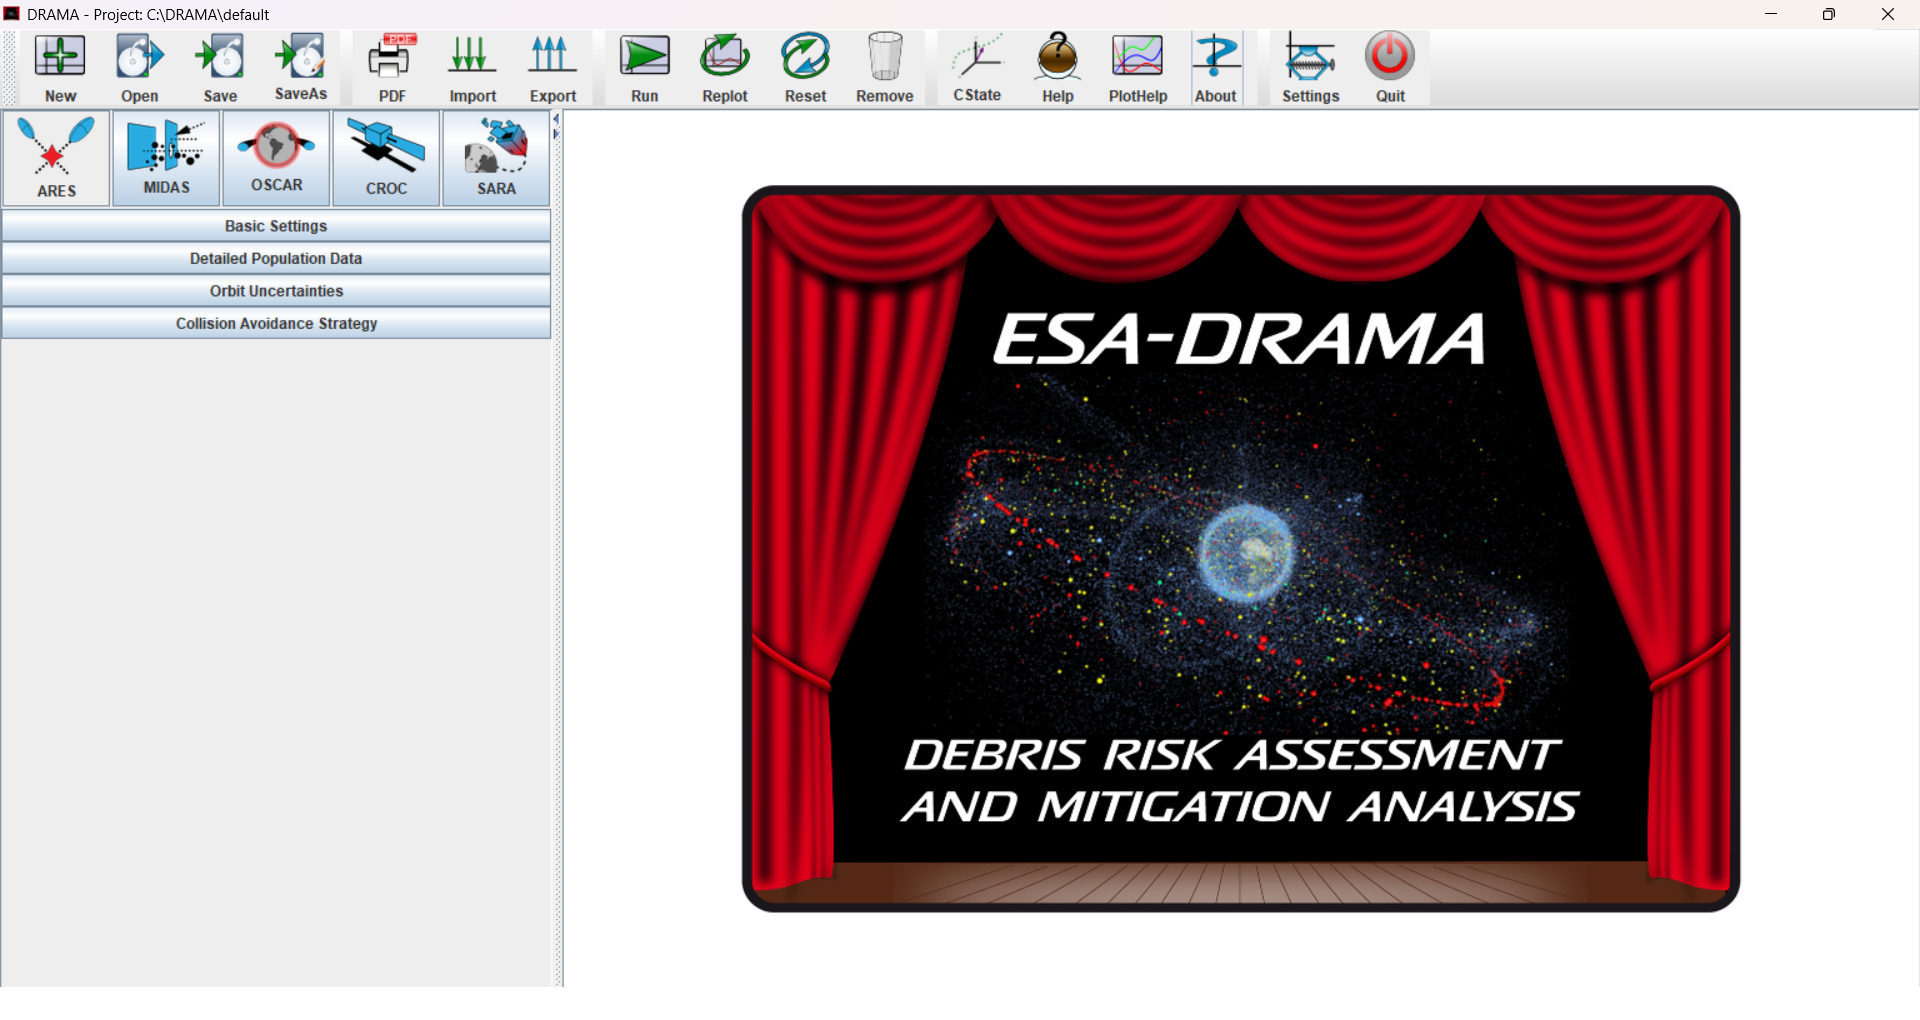
\includegraphics[scale=0.25]{img/drama_mainwindow.png}
%     \caption{Main window of DRAMA}
%     \label{drama_main_window_fig}
% \end{figure}
    \chapter{Satellite Constellation Management Tools} \label{chapter_tools}
This chapter presents all the scripts designed along this work to achieve the purposes of the thesis.
The first paragraph contains the primary functions needed for the development of the main tools proposed from section \ref{revisit_time_collector_par} to \ref{differential_drag_control_par}.


\section{Orbit Propagators} \label{orbit_propagators_par}
The study of the applications and topics covered by this thesis clearly require an orbital propagator.
The core of all the propagators produced along this work exploit the Cowell's model shown in subsection \ref{orbit_prop_paragraph}.
Both undisturbed and perturbed motion have been analysed.

Orbit propagators must take in input the following data:
\begin{itemize}
    \item \textbf{Initial orbit}. The initial state of the staellite orbit must be defined before propagation.
          All the six orbital elements (see subsection \ref{sat_state_rep_paragraph}) and the epoch are required. 
          The scripts can also work defining the six components of position and velocity vectors.
          Even the TLE can be set as input, which will be appropriately converted into the classical elements representation.  
          The reflectivity coefficient must be added if the problem takes into account the SRP.
    \item \textbf{Time settings}. These input parameters include \textit{time frame} and \textit{time step}.
          The first one simply consists of the total temporal period of propagation requested by the user.
          On the other hand, the time step is strictly related to the output density.
          Lower values imply more detailed results, as well as longer computation times.
          In a nutshell, the outputs will be discretized in as many points as those deriving from the ratio between time frame and time step.
          Small time steps provide narrower plots. 
          Figure \ref{time_step_fig} shows the SMA of a LEO satellite under drag perturbation during one orbit (around 50 minutes). 
          The assigned time step is of 5 minutes (the curve is therefore discretized into 10 points).
          It is important to underline that the accuracy of the integrator used by thesis does not depend on this time step value at all.
    \item \textbf{Perturbations parameters}. Propagators that involve any perturbing acceleration need the parameters which describe that force. 
          For example, the perturbing specific force of atmospheric drag (equation \ref{eq:drag_acc}) requires the air density, which will be given by a specific atmospheric model.
          Even for the acceleration of an eventual thruster it is necessary to specify the force it generates.
    \item \textbf{Spacecraft specifications}. According to the features of the selected propagator, one or more satellite characteristics shall be provided when considering perturbations.
          For instance, in presence of atmospheric drag, $C_D$ and $BC$ (which means cross-sectional area and mass) are needed. 
    \item \textbf{Relative tolerance}. It represents the admitted percent error at any step of the simulation. 
          For instance, a relative tolerance of 0.01 indicates a 1\% allowable error limit relative to each state value at each step.
          This setting controls the accuracy of the solution of the selected integrator \cite{rocha2018numerical} (DOPRI$8_{(5,3)}$ is the method used by the thesis).
\end{itemize}

\begin{figure}[h]
      \centering
      %\textbf{Your title}\par\medskip
      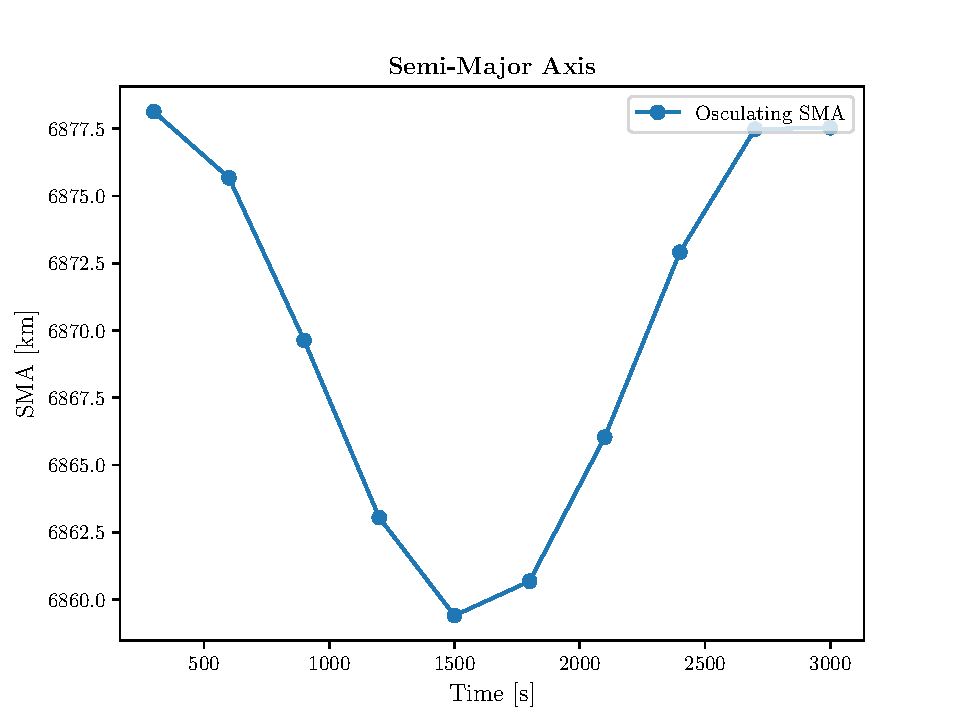
\includegraphics[scale=0.8]{img/time_step.pdf}
      \caption{Osculating SMA of a LEO satellite during one orbit. Propagation time settings: time step = 5 minutes, time frame = 50 minutes.}
      \label{time_step_fig}
  \end{figure}

\subsection{Undisturbed Motion}
The first orbit propagator proposed by this thesis consists of the ideal motion of a spacecraft neglecting all the possible perturbations that might affect it.
Therefore, this kind of propagation is governed by the two-body equation shown in subsection \ref{twobody_par}.

This model is mainly useful for two reasons.
First, it requires computation times definitely shorter than a perturbed propagation, allowing quick results when perturbations are not considered decisive for the purposes of the user.
Secondly, it provides an educational method to better understand the perturbing effects when compared to more realistic propagators.

Figure \ref{kep_low_ecc_fig} shows the orbital elements values of the motion of a satellite in LEO.
\begin{figure}[h]
      \centering
      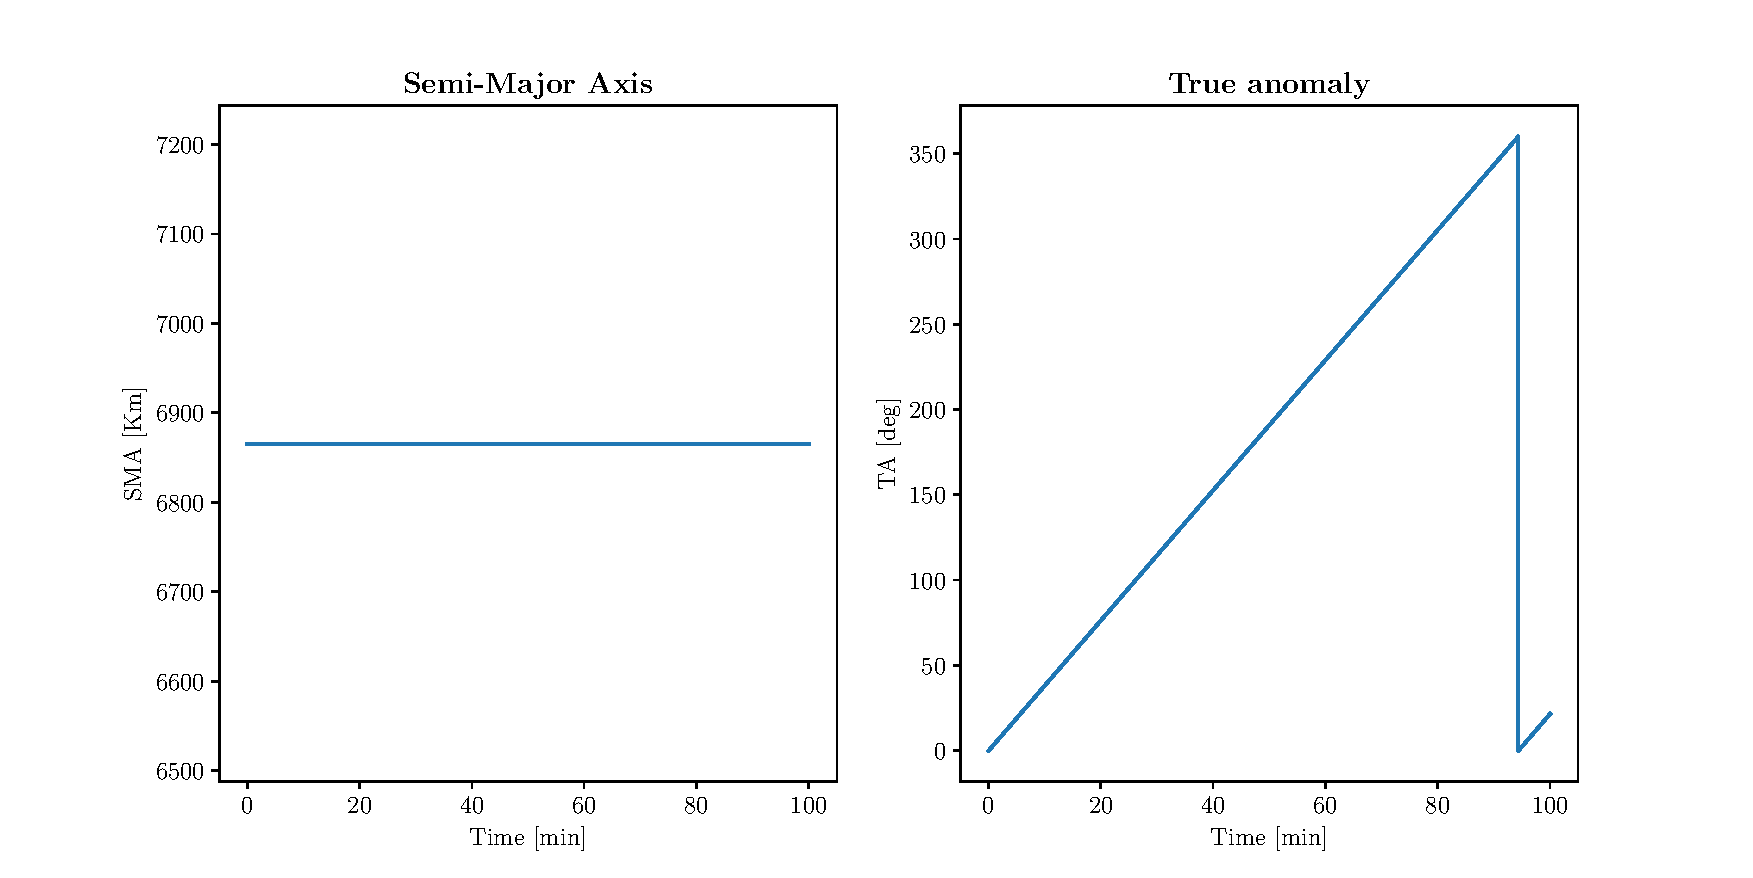
\includegraphics[scale=0.5]{img/keplerian_elements_low_ecc.pdf}
      \caption{SMA and true anomaly variation along around one LEO satellite orbit with eccentricity of 0.001}
      \label{kep_low_ecc_fig}
\end{figure}
Only SMA and true anomaly are reported for matters of layout.
The graph of the other elements is constant like the semi-major axis, because no perturbation affects their behavior.
The true anomaly is the only time-variant parameter, and in this case its curve looks like varying constantly.
The reason of this aspect lies in the eccentricity: this example is characterized by a near-circular orbit, therefore the velocity of the satellite is almost the same along the entire orbit.
Increasing the eccentricity value, like in figure \ref{kep_high_ecc_fig}, the true anomaly changes more rapidly when is in proximity of the perigee and vice-versa.
\begin{figure}[h]
      \centering
      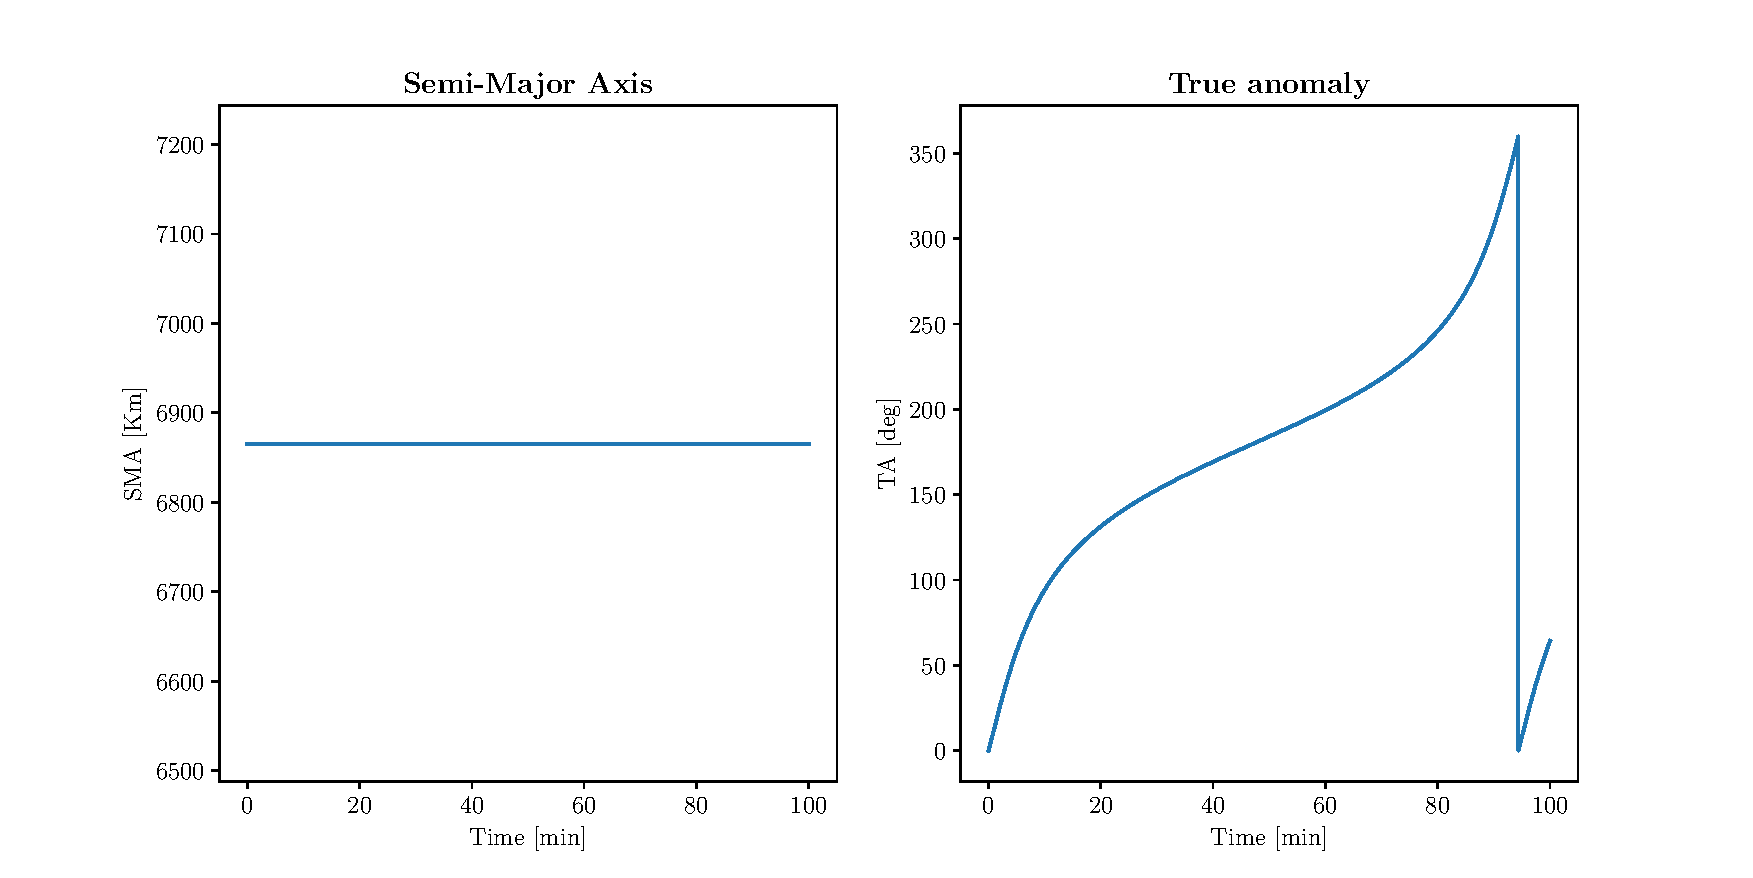
\includegraphics[scale=0.5]{img/keplerian_elements_high_ecc.pdf}
      \caption{SMA and true anomaly variation along around one LEO satellite orbit with eccentricity of 0.5}
      \label{kep_high_ecc_fig}
\end{figure}

All the case studies of this research consist of near-circular orbits.
Despite the fact that zero-eccentricity condition is not feasible, this comparison demonstrates that very low values of eccentricity would make the assumption of circular orbit highly acceptable.
Therefore, the Edelbaum-Kechichian formulas (paragraph \ref{station_keeping_par}) adopted for the station-keeping maneuvers are largely suitable for the problems addressed along the thesis.  


\subsection{Perturbed Motion}
The propagators developed by this work which take into account perturbing effects are based on the Cowell's technique of subsection \ref{orbit_prop_paragraph}.

Since Sun-synchronous orbits at low altitudes denote the main discussion point of this thesis, Earth's oblateness and atmospheric drag represent the perturbations of greatest interest. 
Despite this, propagations with SRP and 3rd-body forces have been examined as well for assessing long-term effects. 

The perturbing acceleration functions performed by this thesis come from the poliastro's library.


\subsubsection{Atmospheric Models}
The atmospheric drag exponential model provided by poliastro has been found to be too approximate compared to the results obtained by GMAT of equal examples.
For this reason, two more accurate atmospheric models have been implemented into the scripts designed along this work.
The first one consists of COESA76 model, while the second is the JB2008 one.
Their theoretical background has been already exposed in paragraph \ref{orbit_prop_paragraph}.
JB2008 is definitely the most accurate model


\subsubsection{Mean Orbital Elements Converter}


\subsubsection{Sun Synchronous Orbits Functions}


\subsection{Satellite Constellation Propagator}



\section{Differential Drag Controller} \label{differential_drag_control_par}
The differential drag algorithm represents the main effort of this thesis.
It consists of a method to perform the phasing through the differential drag of two or more satellites, of any shape and mass, after their deployment at the beginning of the mission.
The goal is to achieve an assigned orbital slot and same mean semi-major axis respectively on all spacecraft forming the constellation, resulting in zero relative velocity between them.
Since the algorithm designed by this thesis takes inspiration from the controller adopted by Planet (Foster et al. \cite{foster2015orbit}), a description of the latter is presented.

\subsection{Planet's Control Algorithm} \label{planet_algorithm_par}
The objective of Planet's algorithm is the same as that of the thesis.
The technique consists of labeling the satellite in the lowest orbit as the leading satellite.
Then, a two-component state composed by the mean Earth-centered angular distance to its desired slot $\theta_i$, and the angular velocity $\dot{\theta}_i$ relative to the leader, is computed for each trailing satellite.
The procedure to achieve the wanted pattern is reported below in the identical form presented by the company \cite{foster2015orbit}.

\begin{algorithm}[H]
      \caption{\textbf{Planet's Control}}
      \begin{algorithmic}[1]
            \Procedure{Create high-drag windows}{} 
                  \State remove any previously issued high-drag windows
                  \State compute $\theta_i$, $\dot{\theta}_i$ of each satellite \textit{i} relative to previous leader (mean, not osculating)
                  \State compute $\ddot{\theta}$ of a satellite in high-drag vs. low-drag mode
                  \State assign leader to be satellite with greatest $\dot{\theta}$ (i.e. lowest altitude)
                  \For{each satellite \textit{i} that is not the leader}
                        \State offset $\theta_i$, $\dot{\theta}_i$ to be relative to new leader: $\theta_i = \theta_i - \theta_{leader}, \dot{\theta}_i = \dot{\theta}_i - \dot{\theta}_{leader}$
                        \State get required high-drag duration to null relative speed with leader: $\Delta t_{i,hd} = - \frac{\dot{\theta}_i}{\ddot{\theta}}$
                        \State get angle travelled during desired high-drag window: $\theta_{i,hd} = \frac{1}{2} \ddot{\theta} \Delta t_{i,hd}^2$
                        \State get wait time to target desired slot: $\Delta t_{i,wait} = \frac{\theta_{i,hd} - \theta_i}{\dot{\theta}_i}$
                        \State create high-drag window for satellite \textit{i} starting at $t_{now} + \Delta t_{i,wait}$ for duration $\Delta t_{i,hd}$
                  \EndFor
            \EndProcedure
      \end{algorithmic}
\end{algorithm}

The strategy is to first obtain the high-drag time $\Delta t_{i,hd}$ (high-drag window) needed by the trailing satellite for matching the leader's semi-major axis, and then the amount of time $\Delta t_{i,wait}$ each spacecraft has to wait in the low-drag configuration before the high-drag maneuver is initiated.

Despite this method has successfully worked for the initial orbit phasing of a satellite constellation, it presents some limitations and ambiguities.
The durations $\Delta t_{i,wait}$ and $\Delta t_{i,hd}$ are predicted making assumptions related to the density of the atmosphere and the attitude of the vehicles.
This leads to unavoidable errors in accuracy.
In addition, it is not clear how the angular acceleration $\ddot{\theta}$ is estimated.
The angle $\theta_{i,hd}$ might also contain inaccuracies because is computed via Taylor approximation.
The accuracy of the algorithm is then strongly sensitive to the initial conditions of dispersion.
Too small differences between satellite orbits do not allow the control to function properly, as well as too big variations lead to inaccurate results.
Despite these negative observations, this algorithm has successfully worked for the initial phasing of a satellite constellation.
The Taylor approximation seems to be quite effective according to the on-orbit results shown in figure \ref{planet_orbit_results_fig} \cite{lee2017cubesat}.
The curves on the graph represent the relative angular distance between each satellite and the leader (which remains at zero degrees in the plot), and the blue lines are the high-drag windows.  
Indeed, Planet reruns its algorithm on a regular cycle to minimize the errors deriving from the forecast of the future state of the atmosphere.
As for the initial dispersion, it can be adjusted always through differential drag maneuvers, in order to achieve more proper initial conditions for the controller \cite{foster2015orbit}.
However, there is no clear information about the appropriate circumstances which make the algorithm work correctly.

\begin{figure}
      \centering
      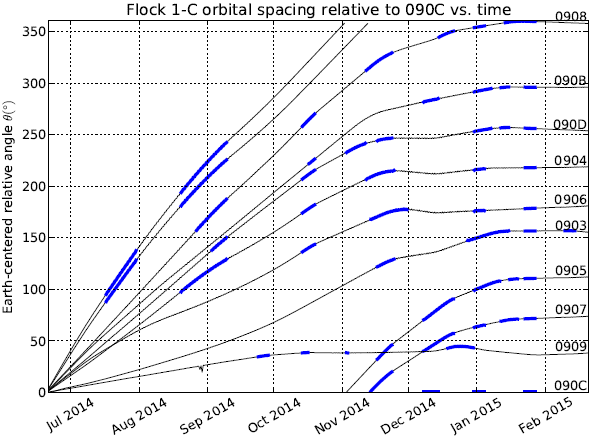
\includegraphics[scale=0.7]{img/planet_orbit_results.png}
      \caption{Actual Planet's fleet relative motion achieved by using differential drag. 
      Blue lines represent high-drag windows \cite{foster2015orbit}.}
      \label{planet_orbit_results_fig}
\end{figure}

Planet has applied this tool to groups of propulsion-less spacecraft.
Once the desired formation is achieved, the same differential drag control is used to maintain the requested relative angular distances between the vehicles.



\subsection{Thesis Controller}
This paragraph contains the work carried out to achieve the main goal of this thesis: the design of a differential drag controller for the initial orbit phasing of a group of spacecraft.
This is then combined with a low-thrust relative station-keeping.
Their coupling enables the orbital management of a LEO SSO constellation of low-thrust satellites throughout the mission lifetime. 
The drag control derives from an improvement of the Planet's algorithm.

First essential requirement is the use of the mean orbital elements.
All the space vehicles involved are supposed to have the same initial orbital elements except SMA and argument of latitude, and all the operations require the use of the mean orbital elements.

The algorithm establishes a reference vehicle, the \textit{leading satellite}, which is identified by the spacecraft travelling in the lowest orbit (greatest mean motion $n$).
The \textit{trailing satellites} have the task of reaching the desired relative placement with respect to the leader.
For each of them, the script computes the distance from the leader by the mean motion, the angular error $\theta_{err}$ from their position to the relative target, and the first attempt value of $t_{est}$.
Angular separations are calculated in terms of argument of latitude.
The latter parameter represents the interval of time in which the algorithm evaluates the variation of $n$.
$\dot{n}$ derives from the acceleration generated by the switch from low-drag to high-drag configuration.
This lead to the assessment of $t_{hd}$, the high-drag window.
After that, the algorithm evaluates the path travelled in high-drag configuration $\theta_{hd}$ and finally the wait time $t_{wait}.$ 
At this point, the estimation of $t_{hd}$ and $t_{wait}$ is repeated with a new $t_{est}$ provided by a function which depends on the altitudes of the satellites and the time intervals computed before.
The procedure is rerun for a sufficient number of iterations.
The procedure is shown below.

\begin{algorithm}[H]
      \caption{\textbf{Differential Drag Control}}
      \begin{algorithmic}[1]
            \Procedure{Perform phasing through differential drag}{} 

                  \State establish the leading satellite (greatest mean motion)

                  \For{each trailing satellite of the constellation}

                  \State compute difference in mean motion with respect to the leader $\Delta n$
                  \State compute angle to reach the desired slot relative to the leader $\theta_{err}$ 
                  \State assign first attempt value to $t_{est}$ from $\theta_{err}$  
                                        
                        \For{assigned number of iterations}
                              
                              \State get mean motion variation $\dot{n}$ from low to high drag mode over $t_{est}$
                              \State get high drag time window $t_{hd} = \frac{\Delta n}{\dot{n}}$
                              \State get angle travelled during high drag window $\theta_{hd} = \frac{1}{2}\dot{n}t_{hd}^2$
                              \State get waiting time window $t_{wait} = \frac{\theta_{err} - \theta_{hd}}{\Delta n}$
                              \State get new estimation time $t_{est} = f(t_{wait}, t_{hd}, h_{lead}, h_{trail})$ 
                        \EndFor
                  \EndFor
            \EndProcedure
      \end{algorithmic}
\end{algorithm}

The strong point of the proposed method lies in the last line.
The estimation time is a critical factor in terms of accuracy for the final result.
It is estimated thanks to an empirical equation formulated within this thesis work.
This function enables a significant better prediction of the two time windows, making unnecessary the rerun of the algorithm in several cases.
Despite this, regular repetition of the calculations remains a good and sometimes necessary action as for the Planet's strategy.
$t_{est}$ is evaluated for an assigned number of iterations, but the experience shows that just twice in enough.
The statements above as will be proven in chapter \ref{results_chapter}.
Similarly to Planet's algorithm, this method is sensitive to the initial dispersion after the deployment.
However, this is issue is easily addressed implementing preliminary high-drag or wait windows.
The only determining factors of this problem are the initial difference in semi-major axis and the altitude from which the launcher deploys the satellites.
The first condition is managed with proper high-drag maneuvers.
On the other hand, when the deployment altitude it is too high, differential drag is unavoidably too low.
Therefore, a preparatory wait time window might be required for the entire fleet of spacecraft, eventually applying high-drag mode to them in order to speed up the process.



\section{Station-Keeping Simulator} \label{sk_simulator_par}
This tool is an absolute station-keeping simulator.
It is able to simulate actions of IAM and DMU performed by low-thrust propelled satellites.
The method combines an orbit propagator and an algorithm that keep the spacecraft within a defined range of altitudes and inclinations.
The required input parameters include the thrust force of the propulsion system as well as the edge values of the orbital elements that define the station-keeping box (paragraph \ref{station_keeping_par}).
The simulator works with the perturbations, therefore it is indispensable to deal with the mean orbital elements to carry out the maintenance.

The logic behind the method is shown below.
\begin{algorithm}[H]
      \caption{\textbf{Station-Keeping Simulation}}
      \begin{algorithmic}[1]
            \Procedure{Simulate the absolute station-keeping of a spacecraft}{} 
                  \For{each time step in the time frame}
                        \State propagate the satellite's orbit
                        \If{current mean SMA < lower SMA}
                            \While{current mean SMA < upper SMA}
                                \State activate thruster
                            \EndWhile
                        \EndIf           
                        \If{current mean inclination < lower inclination value}
                            \While{current mean inclination < upper inclination value}
                                \State activate thruster
                            \EndWhile
                    \EndIf
                  \EndFor
            \EndProcedure
      \end{algorithmic}
\end{algorithm}

The algorithm uses the Edelbaum-Kechichian theory reported in subsection \ref{station_keeping_par}.
However, a careful observer would notice that actually the script takes advantage of this theory only to compute the yaw angle (equation \ref{yaw_angle_equation}) in case of out-of-plane maneuver (change in inclination).
Indeed, the burning time estimated by the equations is never taken into account.
The update of the satellite's position at each time step allows a better accuracy which otherwise would be affected by the uncertainties generated by the unpredictable factors of the perturbing effects over a long time interval.

Nevertheless, the equations of the Kechichian's method are used to provide the $\Delta V$ required by the station-keeping, which is a fundamental parameter for the mission designer.



\section{Revisit Time Collector} \label{revisit_time_collector_par}
The revisit time collector (RTC) tool intends to compute the amount of passages of a satellite above a specific position on Earth.
It collects the \textit{access times} of the spacecraft when its target on the ground is within the area delimited by the swath width of the satellite's on-board camera. 
It can work with a single space vehicle or with a constellation. 
In the latter case, the script provides all the access times taking into account every single satellite of the pattern. 

In addition to the input parameters required by the selected propagator (paragraph \ref{orbit_propagators_par}), the RTC needs the target coordinates in latitude and longitude, as well as the swath width of the electro-optical sensor.
The algorithm computes the distance between the sub-satellite point on the ground and the target at each time step.
This calculation is performed considering some meaningful aspects.

The goal of the RTC clearly requires the estimation of the satellite's position in an ECEF reference frame.
If its motion was evaluated with respect to an ECI system, the ground track of the orbit would be always the same after each orbital period.
ECEF coordinates shall be then converted into the geodetic latitude-longitude location of the spacecraft's subpoint in order to proceed with the distance calculation.

The computation of the distance between two points on the Earth surface shall take into account the sphericity of the planet.
To accomplish this condition, the algorithm computes the so-called geodesic distance, which can be defined as the shortest path between two points on the surface of an ellipsoidal model of the Earth. 
As regards the geodetics, the script takes advantage of the method proposed by Karney \cite{karney2013algorithms}.

Summarizing, the algorithm extracts the sub-point latitude and longitude from the ECEF state vector of the satellite and, after that, calculates the geodesic distance with respect to the ground target.
This path is then compared with half the value of the potential swath width (PSW) at each time step of the propagation.
If the distance is smaller than PSW then the script saves the epoch related to that time step.

\begin{algorithm}
      \caption{\textbf{Revisit Time Collection}}
      \begin{algorithmic}[1]
            \Procedure{Collect revisit time epochs over a specific target}{} 
                  \State propagate the satellite's orbit for the desired time frame
                  \For{each time step in the time frame}
                        \State convert satellite state vector from ECI to ECEF
                        \State extract geodetic latitude and longitude
                        \State compute the geodesic distance between target and sub-satellite point
                        \If{distance between the two points < $\frac{PSW}{2}$}
                              \State collect the epoch of the current time step
                        \EndIf
                  \EndFor
            \EndProcedure
      \end{algorithmic}
\end{algorithm}

It is important to underline that the actual sensor input value to be implemented in the RTC should be related to the concept of \textit{potential swath coverage}.
It identifies the potential path reachable by a pointable space system.
If the satellite can not work off-nadir then the input parameter will be simply equal to half the SW due to the fact that the subpoint always lies in the middle of the observed area.
Therefore, according to the figure \ref{potential_sw_fig}, a proper use of the algorithm should get half the potential swath width (PSW) as input value.
\begin{figure}[H]
      \centering
      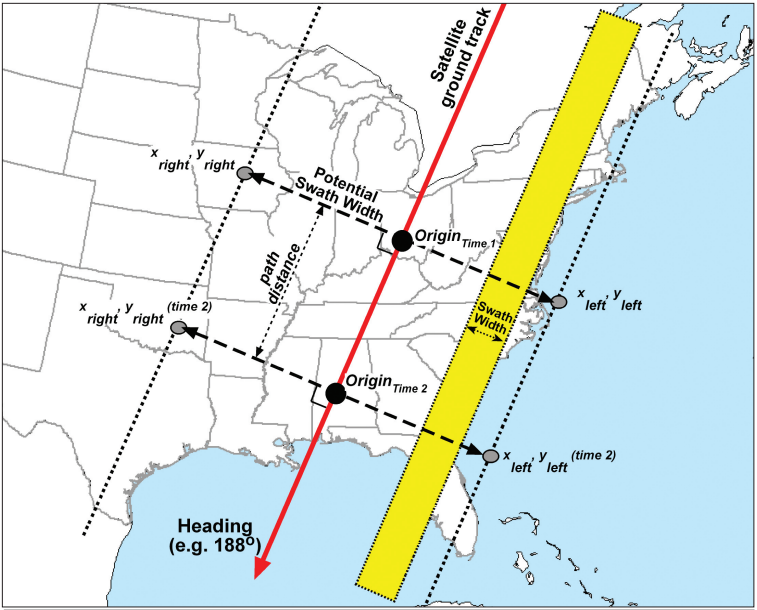
\includegraphics[scale=0.6]{img/potential_sw.png}
      \caption{Projection of satellite ground track and potential swath width with respect to its swath width at two time steps \cite{hodgson2008modeling}.}
      \label{potential_sw_fig}
\end{figure}
    \chapter{Case Studies}

\section{Reaktor Hello World}

\section{Hyperfield Next Generation}

\section{Planet CubeSat Constellation}

\section{Future Kuva Constellation}
    \chapter{Analysis and Results} \label{results_chapter}

\section{Reaktor Hello World Life Data}

\section{Hyperfield Orbit Maintenance Design}

\section{Planet Constellation Differential Drag Results}

\section{Kuva Constellation Management Results}

    \chapter{Conclusion}

\lipsum[23]

  \bibliography{bibliography} % bibliography, sampleBibFile
  \bibliographystyle{unsrt} % acm

\end{document}